\subsection{Results}

\subsubsection{Crop health survey data}

Prior to using the crop health survey data to construct the network, some exploratory plots of the data are constructed and examined. The figure shows the distribution of the data. A total of 415 farmers' fields was surveyed in Tamil Nadu, India (TMN); West Java; Indonesia (WJV), Laguna, Philippines (LAG); Suphanburi, Thailand (SPB) and Mekong river delta, Vietnam (MKD) from 2009 to 2013. Survey field was intensively cultivated, 97\% of which were irrigated and 98\% were planted to modern varieties. The data collected pertain to injuries caused by pathogens, animal pests. The protocol gives more emphasis on the nature of injuries and not on the causal organism. The levels of injuries during a cropping season were computed or summarized according to the nature of injuries and thus varied in scale. For example, foliar disease were summarized as area under the disease incidence progress curve, viral diseases as area under the progress curve of the field area affected, and tiller injuries or diseases as a maximum incidence. 

The injuries caused by animal pests observed during the survey period were rat injury, deadhead and whitehead caused by stem borers, whorl maggot injury, leaffolder injury, gall midge injury (silver shoot). Rat injuries were observed high incidence in MKD in dry season 75\% as an maximum level. They were also observed at WJV in dry season, and both season in TMN, LAG, SPB. Gall midge injuries (silver shoots) in during survey period were not observed in TMN and LAG. They were found in SPB, MKD, but WJV at maximum 25 \%. Deadheart were observed all survey sites. There are more severe in dry season at SPB and MKD, but for WJV and LAG, they are  more severe in dry season. The trend of whitehead incidence observed were opposite the deadheart incidence, which were more server in wet season at SPBm and MKD, but less severe at WJV and LAG. Leaffolder injuries were observed all survey locations. They are more severe in wet season at WJV, TMN, and LAG, but more severe in dry season at SPB, and MKD. Whorl maggot inquiries were observed at all locations. They highly occurred in LAG, and they are more severe in wet season than the wet season at all location except LAG, where their incidence scattered broadly in dry season.

Brown planthoppers were  found all location of survey sites. During the survey period, they are found higher population in wet season than dry season in TMN and MKD, but  there were some observation of BPH other locations. White backed planthoppers were commonly found at MKD in both of dry and wet season, and there are a few observations in WJV and LAG, but at TMN and SPB, they were not observed. Rice bug could be observed all survey location. They were highly found in dry season than wet season at WJV, LAG , and MKD. but in SPB , they were found only in wet season during the survey period.  Green leafhopper were observed all location. They were found in LAG higher than other location.

The disease that were recorded during the survey period were bacterial leaf blight,bacterial leaf streak, brown spot, leaf blast, narrow brown spot, read stripe, sheath blight, sheath rot, false smut, stem rot. BLB were observed all location but high in wet season in SPB.  BLB were higher in dry season than wet season in WJV and MKD, but higher in  wet season in TMN, LAG, SPB. BLS were observed  all location except TMN. they were higher in wet season than dry season. BS were observed inn all location except TMN. they were found higher in wet season than dry season. The highest incident were in Thailand. LB were observed at all location. they were high in MKD in drys season . Other location were found some fields. NBS were found all location except TMN during the survey period. there were many field in SPB found high level of NBS incident. NBS were more severe in wet season than dry season. RS were observed in all location except TMN. there were many fields found high RS incident. DP were found all location except TMN. The high incident were found in MKD. FS were commonly found all location. The hight incidents were observed in SPB, and MKD.NB were observed  at all location. They were found many observation in TMN. S HB commonly found all location.  high incidence in TMN, and LAG.  SHR except TMN, Many observations were higher the value in major observation. SR except TMN. There are a few observation presenting the SR. 

% I still do not know that the interpretation of the network wise propertis
%\paragraph{Network level topological features of seasonal crop health survey}
%There are three features that we will considering the network wise properties.The diameter of a graph is the length of the longest geodesic. From dry to wet season, network complexity is different.India dry season network 

% Please add the following required packages to your document preamble:
\begin{table}[]
\centering
\begin{tabular}{llllllll}
\hline
\multirow{3}{*}{Country} & \multicolumn{6}{c}{year} & \multirow{3}{*}{Total} \\ \cline{2-7}
                         & \multicolumn{2}{c}{2010} & \multicolumn{2}{c}{2011} & \multicolumn{2}{c}{2012} &                        \\ \cline{2-7}
                         & DS         & WS          & DS          & WS         & DS          & WS         &                        \\
\hline
India                    &            & 25          & 60          &            & 20          &            & 105                    \\
Indonesia                & 5          & 20          & 30          & 30         & 20          &            & 105                    \\
Philippines              &            & 20          & 20          &            &             &            & 40                     \\
Thailand                 &            & 20          &             & 45         &             & 40         & 105                    \\
Vietnam                  &            & 20          &             & 15         & 25          &            & 70                     \\
\hline
Total                    & 5          & 115         & 110         & 90         & 65          & 40         & 425    \\
\hline               
\end{tabular}
\caption{Number of farmers' fields surveyed by country and year}
\label{table:Survey_data}
\end{table}

\begin{table}
\centering
\caption{rice production season}
\label{table:rice-production-season}
\begin{tabular}{lllll}
\multicolumn{1}{c}{\multirow{2}{*}{Country}} & \multicolumn{2}{c}{Dry}                                       & \multicolumn{2}{c}{Wet/Winter*}                            \\
\multicolumn{1}{c}{}                         & \multicolumn{1}{c}{Planting} & \multicolumn{1}{c}{Harvesting} & \multicolumn{1}{c}{Planting} & \multicolumn{1}{c}{Harvest} \\
Indonesia                                    & April                        & October                        & November                     & March                       \\
India                                        & November                     & Mar                            & Jun                          & October                     \\
Philipppines                                 & November                     & April                          & May                          & Octber                      \\
Thailand                                     & January                      & June                           & August                       & December                    \\
Vietnam                                      & December                     & April                          & April                        & August                     
\end{tabular}
\end{table}

\subsubsection*{Co - (and anti) occurrence of injury profiles based on network analysis}

The co-occurrence correlations of injury variables were explored using network inference based on strong and significant correlations through using non-parametric Spearman’s rank coefficient at $P$ < 0.05, which indicated that the co-occurring variables have good association. The setup of Spearman's coefficient cutoff could efficiency reduce the sparse correlation and highlight the significant correlation between variables. Therefore, the network were determined for the co-occurrence analysis of injury variables, based on the crop health data in the 10 groups, which were different country and season shown in Fig to Fig. Nodes represent injury variables  and links represent Spearman's correlation coefficients at $P$-value < 0.05. In order for a network model to bolster understanding of a complex system, it is necessary to quantify the topological features or properties of the network. Important properties include:

\begin{itemize}
\item \textbf{Node degree} is the number of neighbors of a node, also known as connectivity. Node (variable) with high degree (many links to other nodes) can be implied that this node has strong connections, and  potentially co-occurs with other nodes. 

\item \textbf{Local clustering coefficient} is a measure of the degree to which nodes tend to cluster together. It is defined as how often a node forms a triangle with its direct neighbours, proportional to the number of potential triangles the relevant node can form with its direct neighbours. In the context of this network, local clustering coefficients is the the probability that two neighbors of  injury variables of the injury variable co-occur with each other in the network.These measures are indicative of the complex forming of co-occurrence patterns through the network. As presented nodes can be observed other nodes, a more closely connected network facilitates nodes co-occurrence.

\item \textbf{Betweenness} is measure the number of paths, which a node is present on the shortest path between all other nodes. Nodes with high betweenness have been shown that there are many pair-wise relationships across a network pass through the node, which is implied that the nodes has high possibility to occur (easily to be induced). 

Moreover, we inspect the community structure of the networks derived from the empirical data, to identify the injury symptoms (the combination of injuries) that are especially highly connected.

\end{itemize}

\ref{table:Network_stat}.

\paragraph{Tamil Nadu, India (TMN)} 


Dry season network (Fig) composed of 6 nodes (injuries, DH, NB, SR, FS, RB, and LF), and captured 7 associations. The network analysis resulted in detection of two groups of injury profiles (the combination of injuries). The groups of the injury profiles corresponded to each communities based on the optimal clustering algorithm. The first group is composed of DH, LF, RB and SR.  Another group consists of FS and NB. Analysis of network properties revealed that one of each group (LF and FS ) has high betweenness, which indicated that they also present co-occurrence relationships within the group, and between groups. So when FS or Lf present in the fields, It is possible to be able to observed the other injuries, which are within same group or different groups. SR and RB have high clustering coefficient, which are implied that these injuries usually formed complex of multi-co-occurrence relationships. As opposed to other injuries, NB and DH have low scores on all three centrality measure. Apparently, injuries variable either are less possibly co-occur with other injuries (low betweenness), and not form multi-co-occurrences with other nodes (low degree and clustering coefficient).


Wet season network (Fig) was composed of 12 nodes (injury variables, DP SR, FS, BLB, NB, LF, GLH, RT, RB, DH, WM, BPH) with edges. Fig reveals three groups of injury profiles. 
DH, GLH, SR and BPH are in the first group (green). FS, NB, DP, BLB is in the second (orange). RT, LF, RB and WM are in the third group (purple). The network properties. Top four injuries with high betweenness are the members of each of group (DP, SR, LF, and BLB). They possibly are found co-occurrence within the group and inter-groups of injury profiles. Considered in each group, DH and GLH have high clustering coefficient in the first group. NB has high clustering coefficient in the second group. RT has highest clustering coefficient comparing other injuries in the group. WM, BPH have low value of the three features, and located . BPH and WM were less possible to occur, and present co-occurrence patterns, and when they were observed, they were also not able to relate to many injuries. 
  

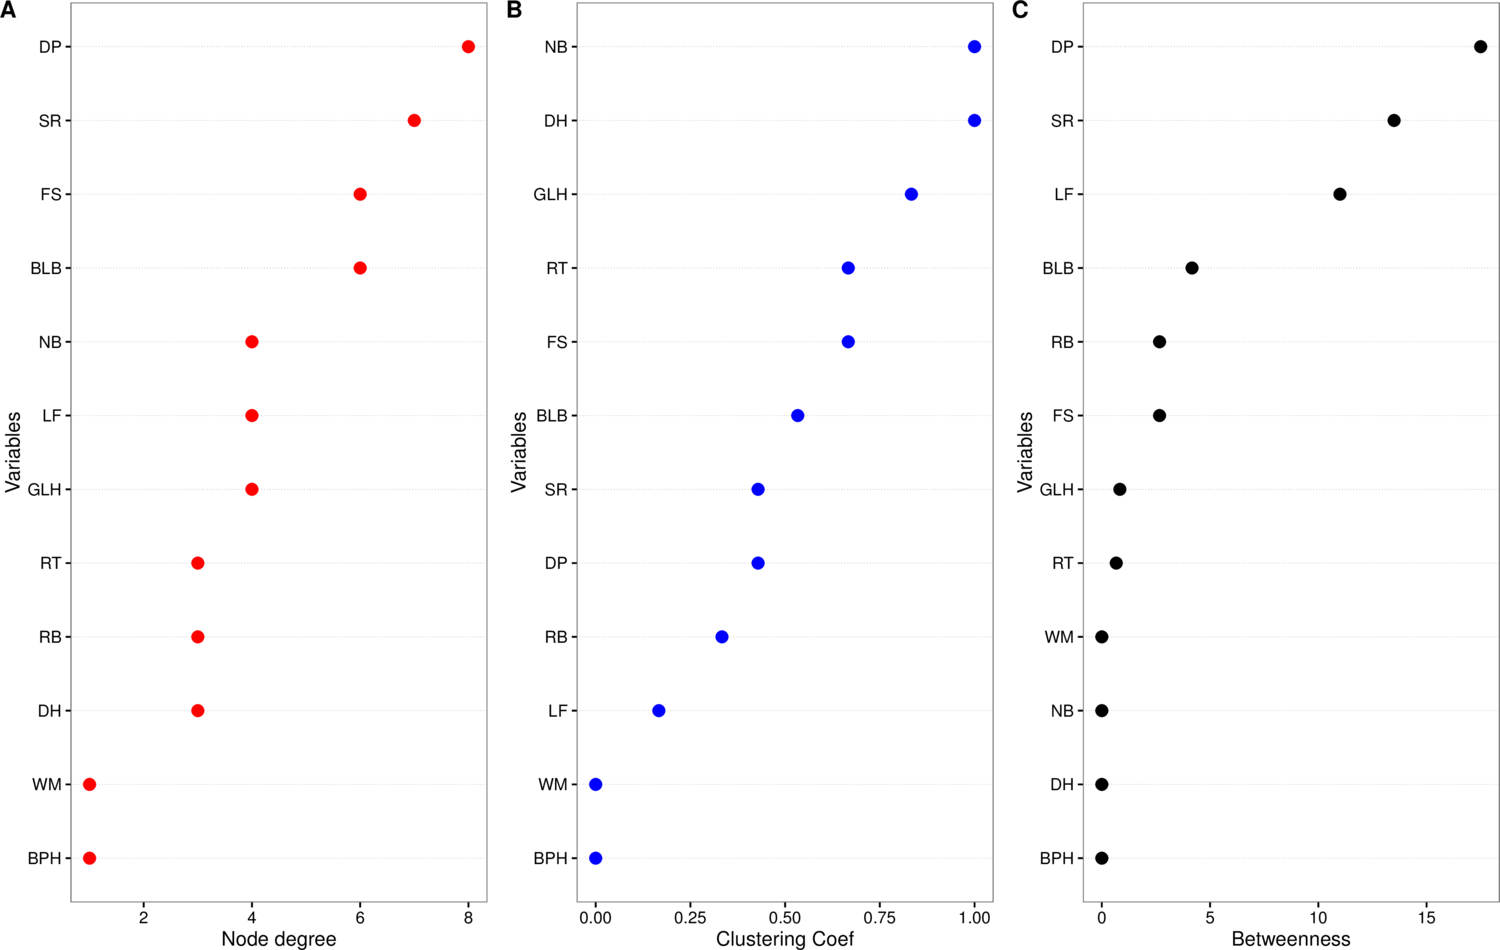
\includegraphics[width=\textwidth]{Network-analysis-/figures/nodepropind_ws/nodepropind_ws.png}


\paragraph{West Java, Indonesia}
 
Dry season network (Fig.) composed of 20 nodes and 51 associations. The network reveals four groups of injury profiles. The first group (green color) include DH and RT. The second group (orange color) include NBS RB, FS, BLS, LB, DP, BLB, NB, BS. The third group (purple color) included GM, LF, BPH, SR, SHB, GLH, RS. The last group (pink color) include WM and WH.  The second and third group are formed closely clusters.  RT in the first group, BLB and BS in the second group,  LF of the third group, and WM in the fourth groups have with high betweenness, and intermediate clustering coefficient.  NBS, NB, RB, BLS, FS, DP of the second group have high clustering coefficients. Compared to the the second group, the injuries in the third group has relatively smaller than. It indicated that the injuries in the second group are tightly formed multi-co-occurrence (not few pairs of co-occurrence).  DH, WH have low value of the three features, and located far from the center of the network. BPH and WM were less possible to occur, and present co-occurrence patterns, and when they were observed, they were also not able to relate to many injuries. 
connectivity.

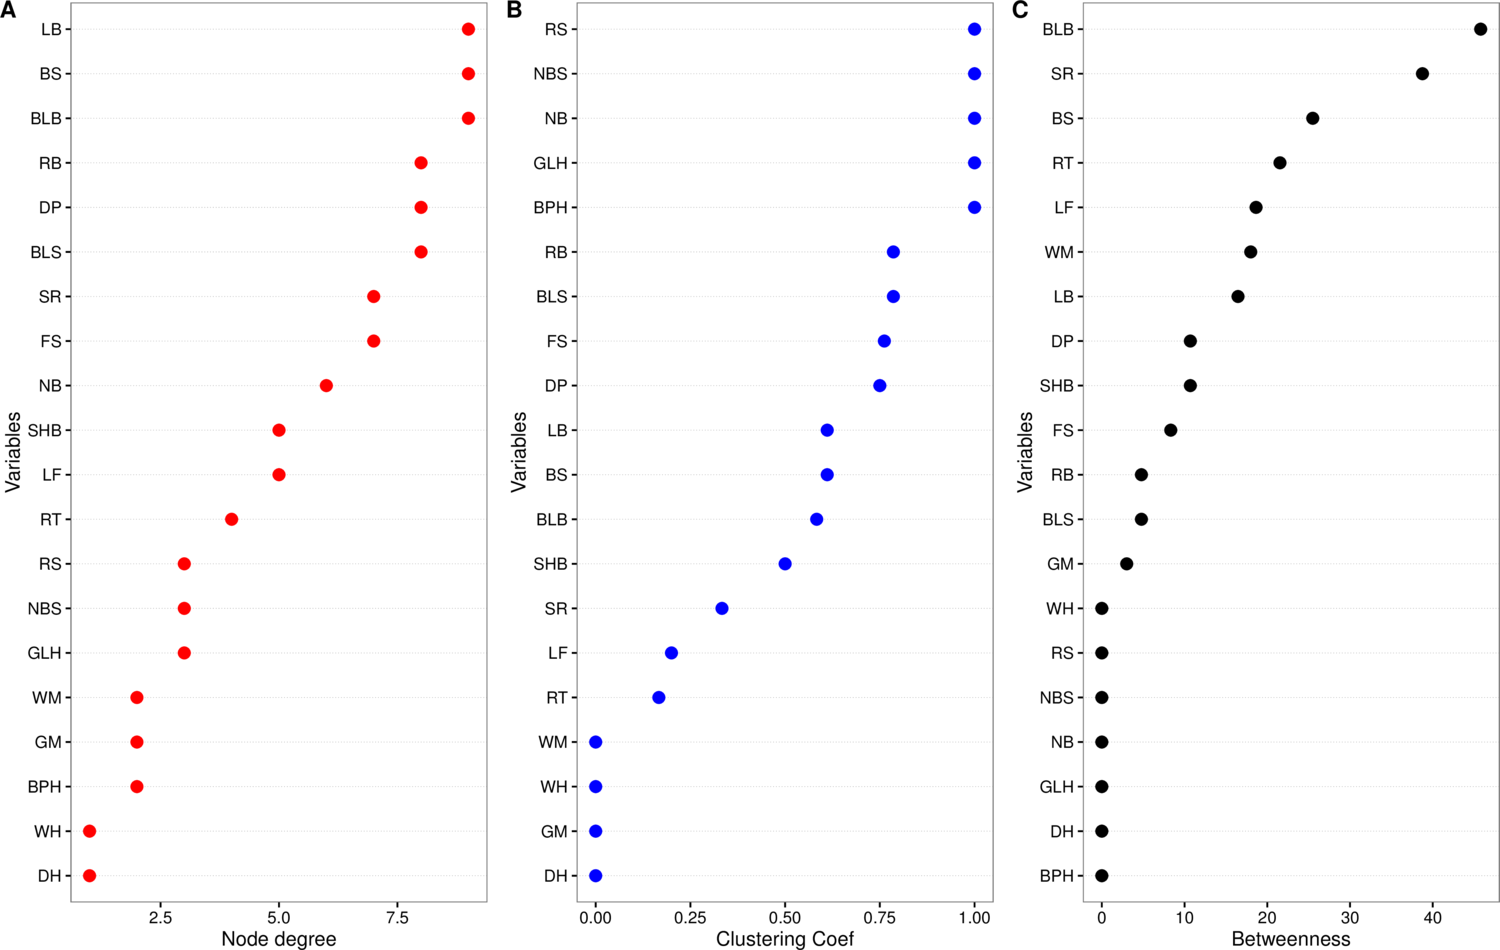
\includegraphics[width=\textwidth]{Network-analysis-/figures/nodepropidn_ds/nodepropidn_ds.png}

Wet season network
Wet season network (Fig.) composed of ? Nodes. (injury variables, WM, LF, GLH, DH, BLS, WH, NBS, FS, DP, RS, LB, WPH, SR, SHR, SHB, NB, BS, BLB) and ? relaships. The network is not formed the closed cluster.   It reveals 4 groups of injury profiles. The first group (green) DH, WM, SHB, WH, GHL, LF, LB, and RS. The second group (orage) is composted of WPH, SR, GM, BLS and DP.  The third group consist of FS, NBS, SHB, BLB. The forth group are BS and NB. The first group is the biggest group of the injuires profile with WM is the injuries with high betweenness, and WH is the injury with high clustering coefficient. The second group has BLS that the node with high betweenness, and DP is the ode with high clustering coefficient. The third group  has FS node with high betweenness and high clustering coefficient. There is separated group, which is composted of BS and NB. The first group is seem to form complex  co-occurrence patterns because the average of clustering coefficient of injuries in this group are higher than other groups of injuries.  
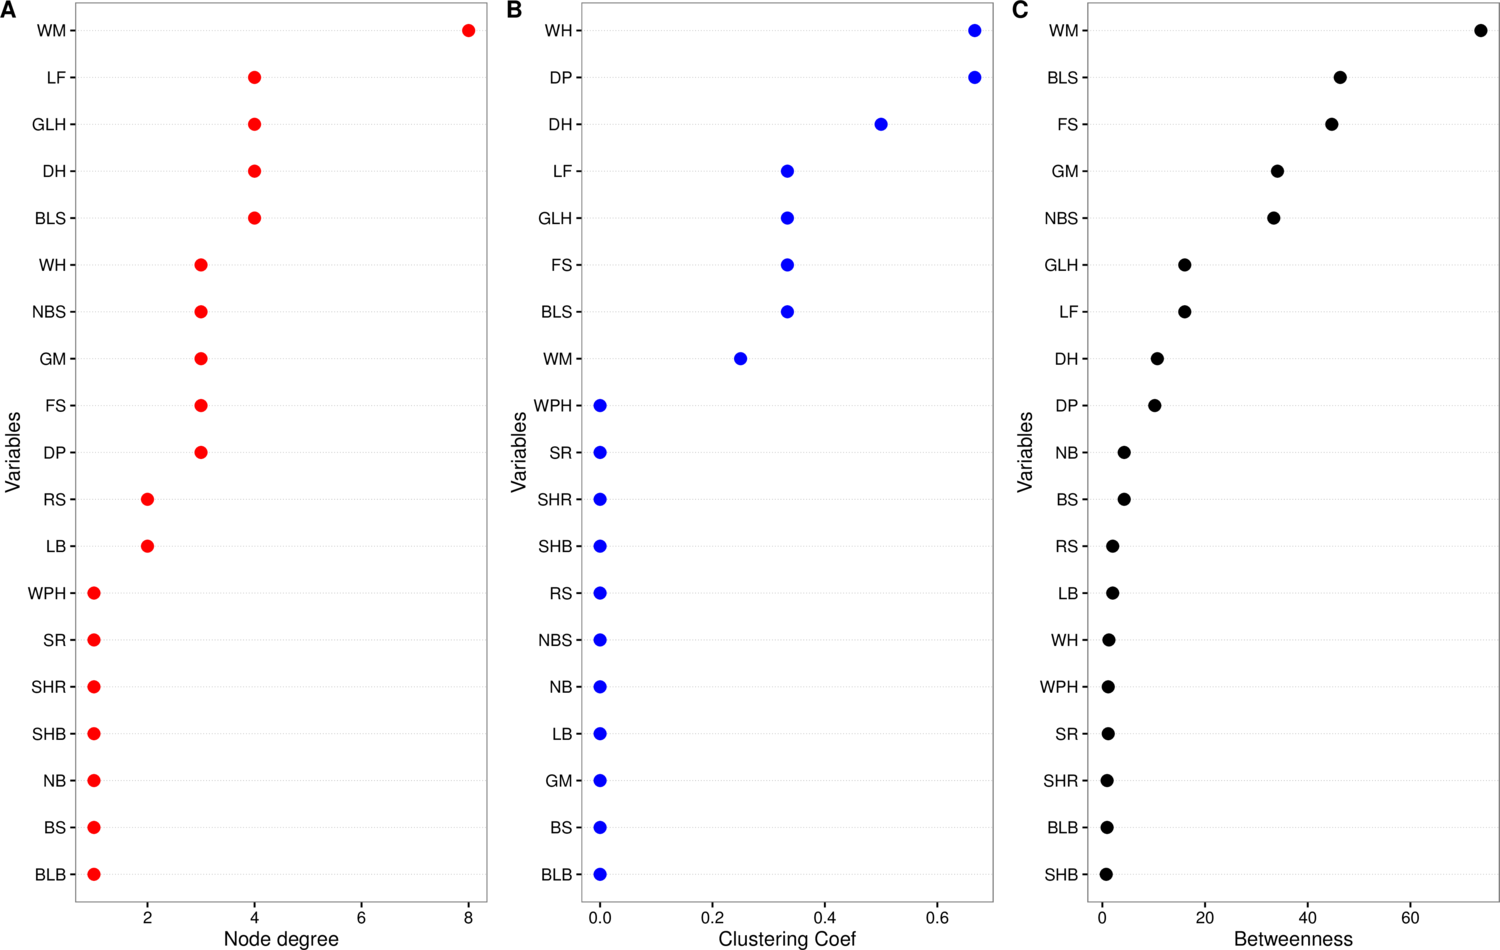
\includegraphics[width=\textwidth]{Network-analysis-/figures/nodepropidn_ws/nodepropidn_ws.png}

\paragraph{Central Luzon, Philippines}

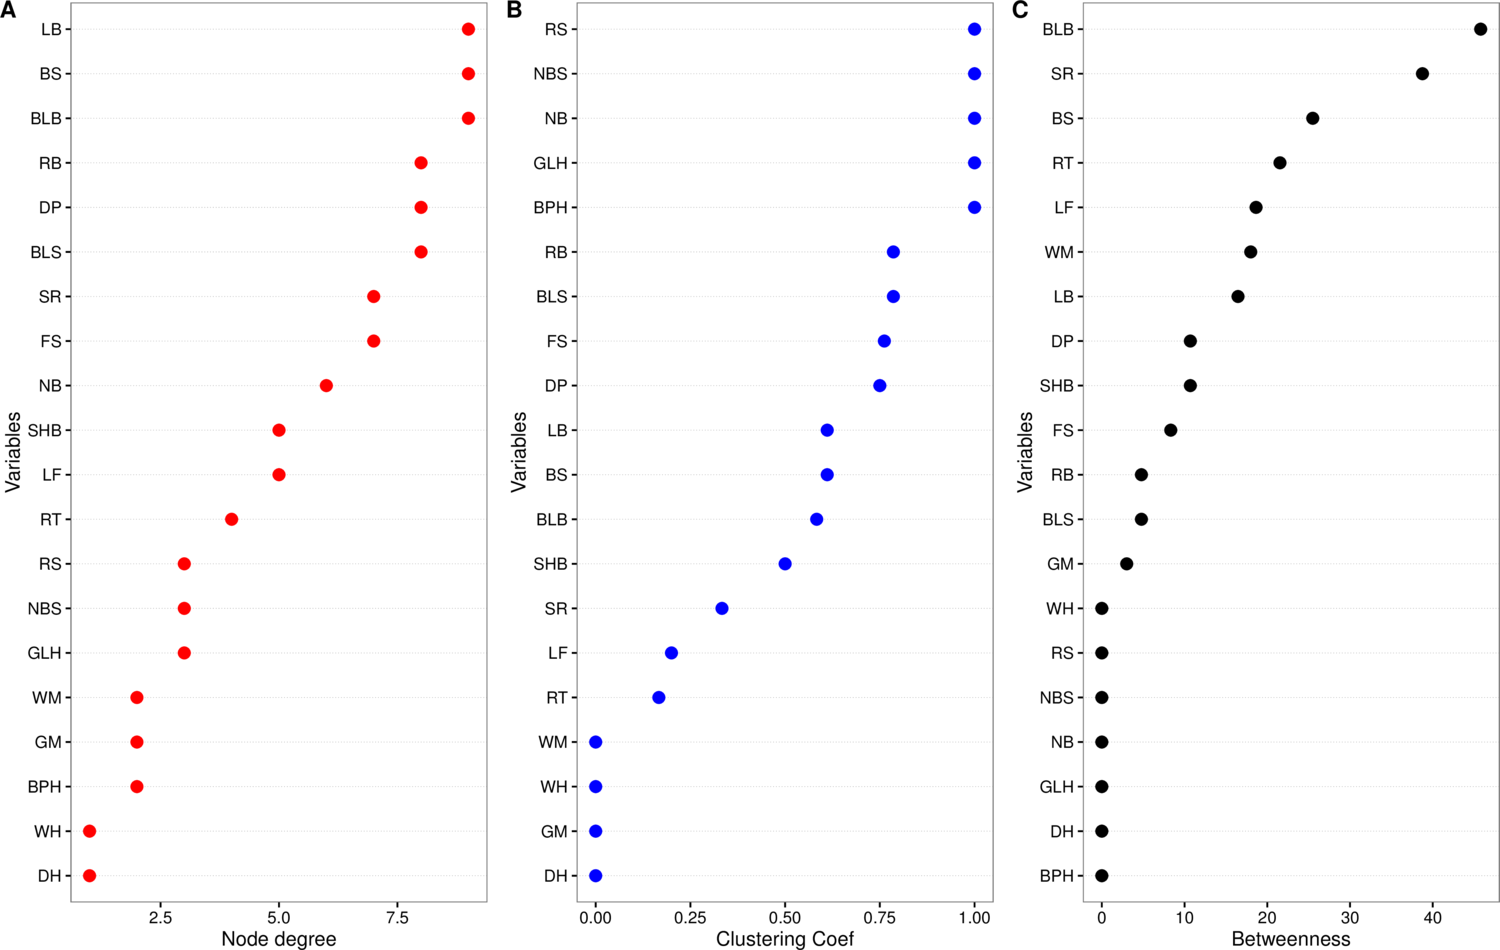
\includegraphics[width=\textwidth]{Network-analysis-/figures/nodepropidn_ds/nodepropidn_ds.png}
The network reveal three groups of injury profiles. The first group composted of WM, RB, NB, SHB, and FS. The second group consist of LB and DP. The third group is GLH, BPH and BLB.  The WM and RB in first group have high rank of betweenness. BPH and DP are also have high rank of betweenness, which are in the second and the third group, respectively. Interestingly, SHB in the first group, and GLH in the third group have high clustering coefficients. The NB, LB, FS, and BLB featured low in three of centrality. 

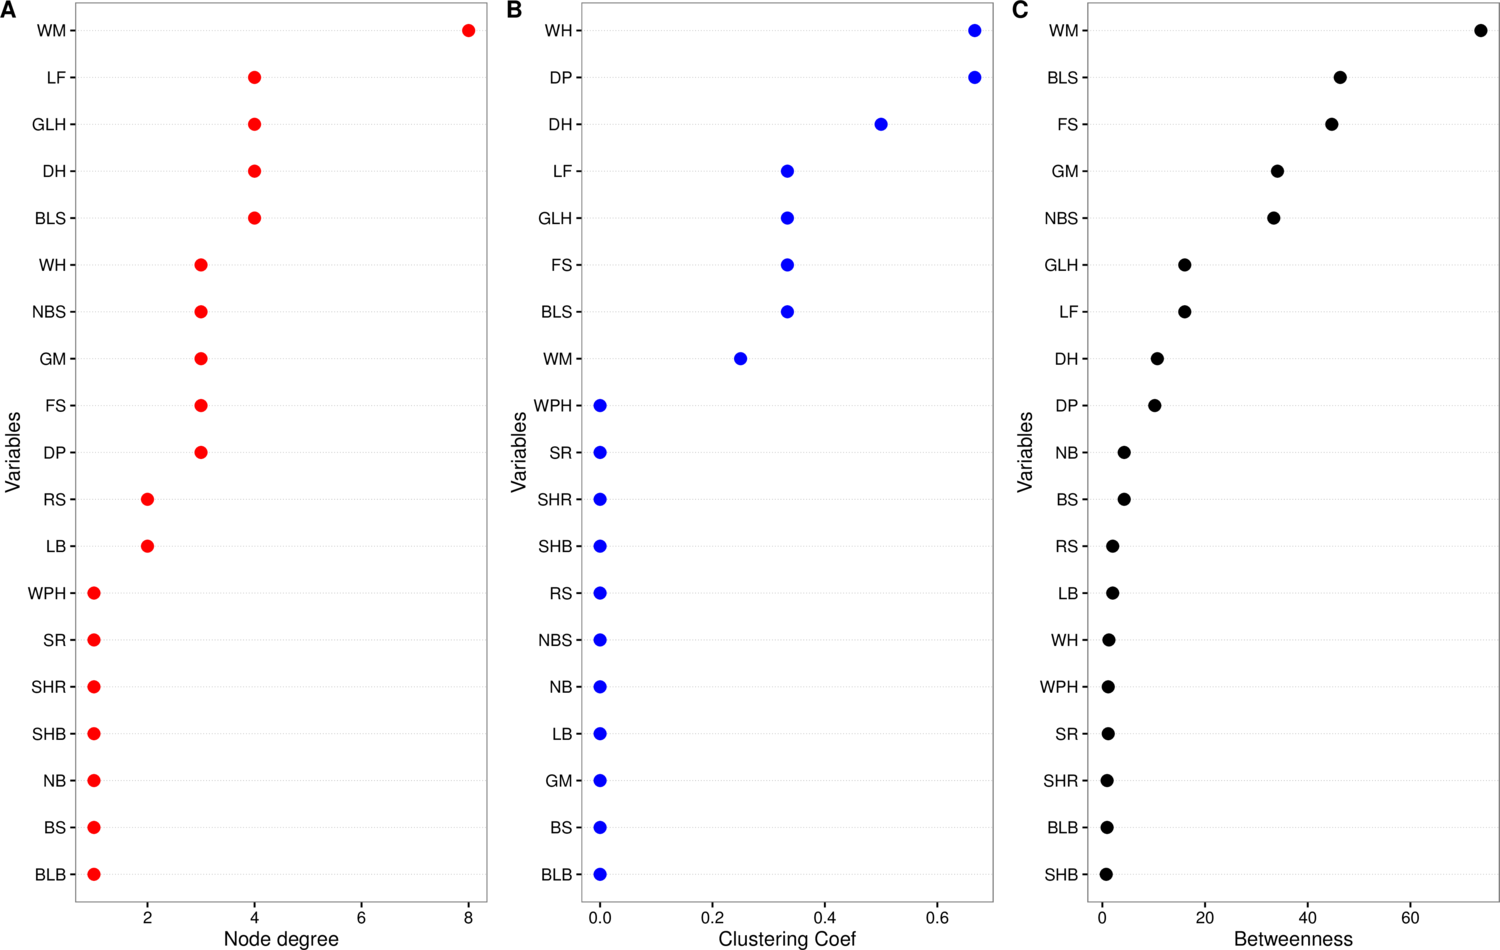
\includegraphics[width=\textwidth]{Network-analysis-/figures/nodepropidn_ws/nodepropidn_ws.png}
Network reveals four groups of injury profiles. The second group (green) has  SHR, RS, RT, which is isolated. The first group (orange) has NB, RB, GLH, BLS, and DP. The third group (purple) has LB, SHB, LB. The forth group (pink) has NBS, LF, BS, and BLB. The first group is more complex combination than others because the clustering coefficients of injuries in this group are higher. Interestingly, the third group is in between the first and the fourth group, this position supported that the injuries express high betweenness. 

\paragraph{Suphan Buri, Thailand}


SUP in dry season the network shows  8 variables (DH, BS, SR, SHB, NBS, SHR, GLH, and WH) showing 12 edges (significant pair-wise relationships).  From the result of community detecting.  We found there are three closed co-occurrence patterns of injuries. The first group (green) is composted of NBS, DH, BS, and SHB. Second patterns (orange) is SHB and GLH, and the Third group ( purple) is SR and WH. The first  one seem more complex than other two group because three out of four node in the groups present high clustering coefficient NBS, DH, SHB,  and SR seem to be clustered together.  BS present high betweenness in the first group, which is associated with the other two groups. SHB has high moderate degree and high betweenness, whereas  it has low betweenness.  It can form complex association with the injuries in the first group and the second group itself.  WH and GLH feature low scores on at least two centrality measures.  Apparently, they are less easily found with other injuries, do not tend to complex combination because of low inter-co-occurrence ( low clustering coefficient), or less possible for expressing co-occurrence through the network (low betweenness). 
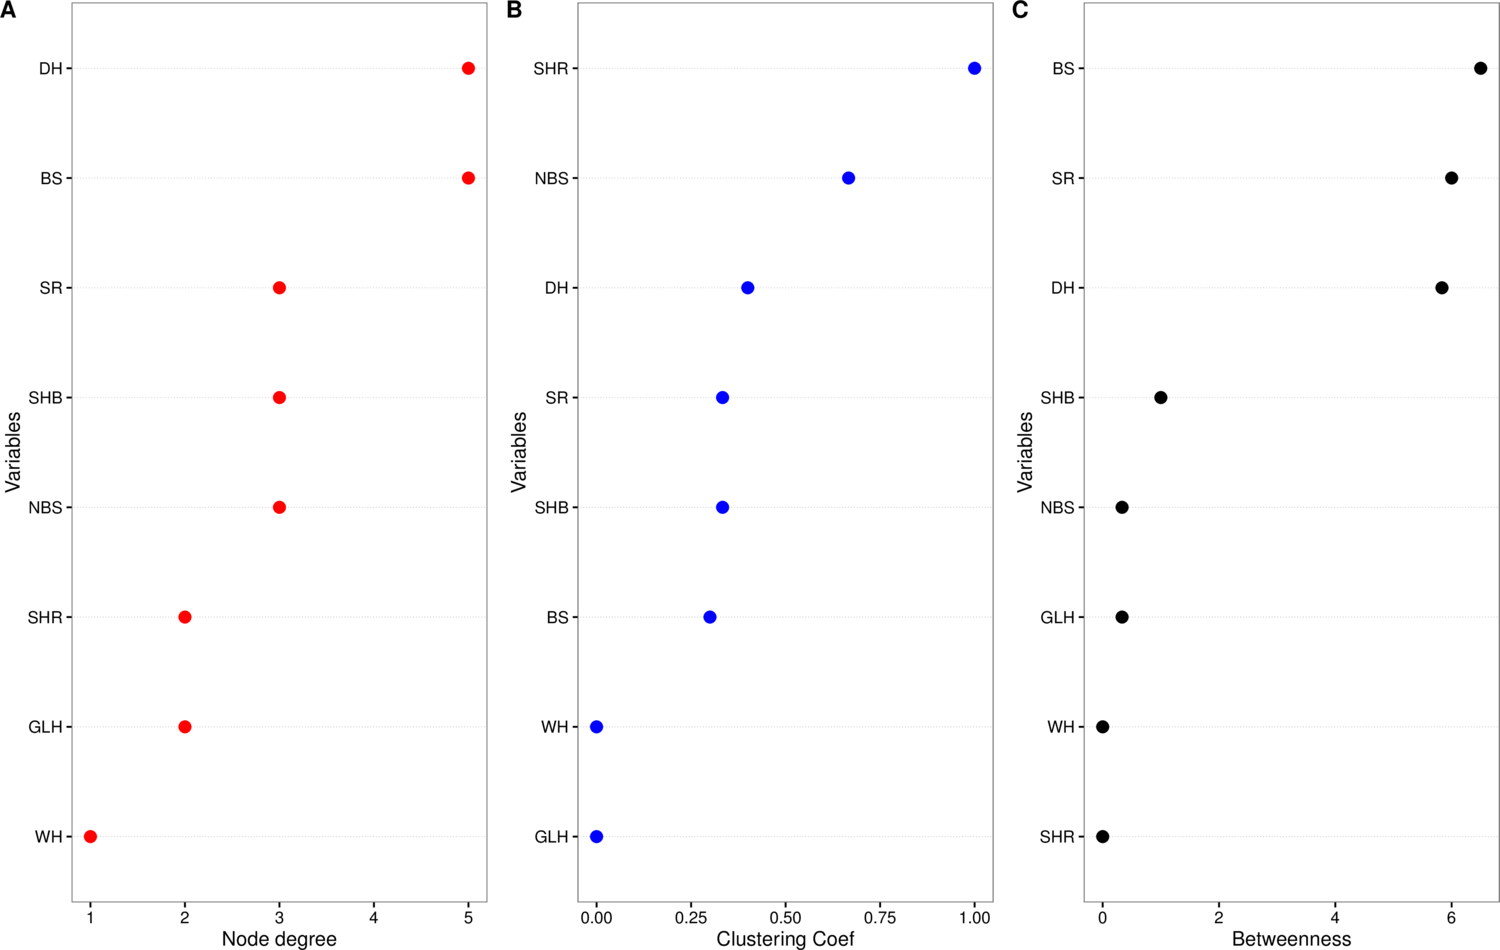
\includegraphics[width=\textwidth]{Network-analysis-/figures/nodeproptha_ds/nodeproptha_ds.png}

SUP in wet season network shows  18  variables (DH, BS, SR, SHB, NBS, SHR, GLH, and WH) showing  79 edges (significant pair-wise relationships). There are three closely clustered groups. The first group (green) composted of NBS, FS, RT, SHB, LB, WM, RS and RB. The second group (orange) consist of GLH, BS, GM, SR, BLB, BLS, LF and DP. The third group consisted of SHR and NB. The first and the second group are formed complex association. Interestingly, SHR in the third group has high betweeneess, which is in-between the association of the injuries between the others and into the groups of the injuries profiles. 
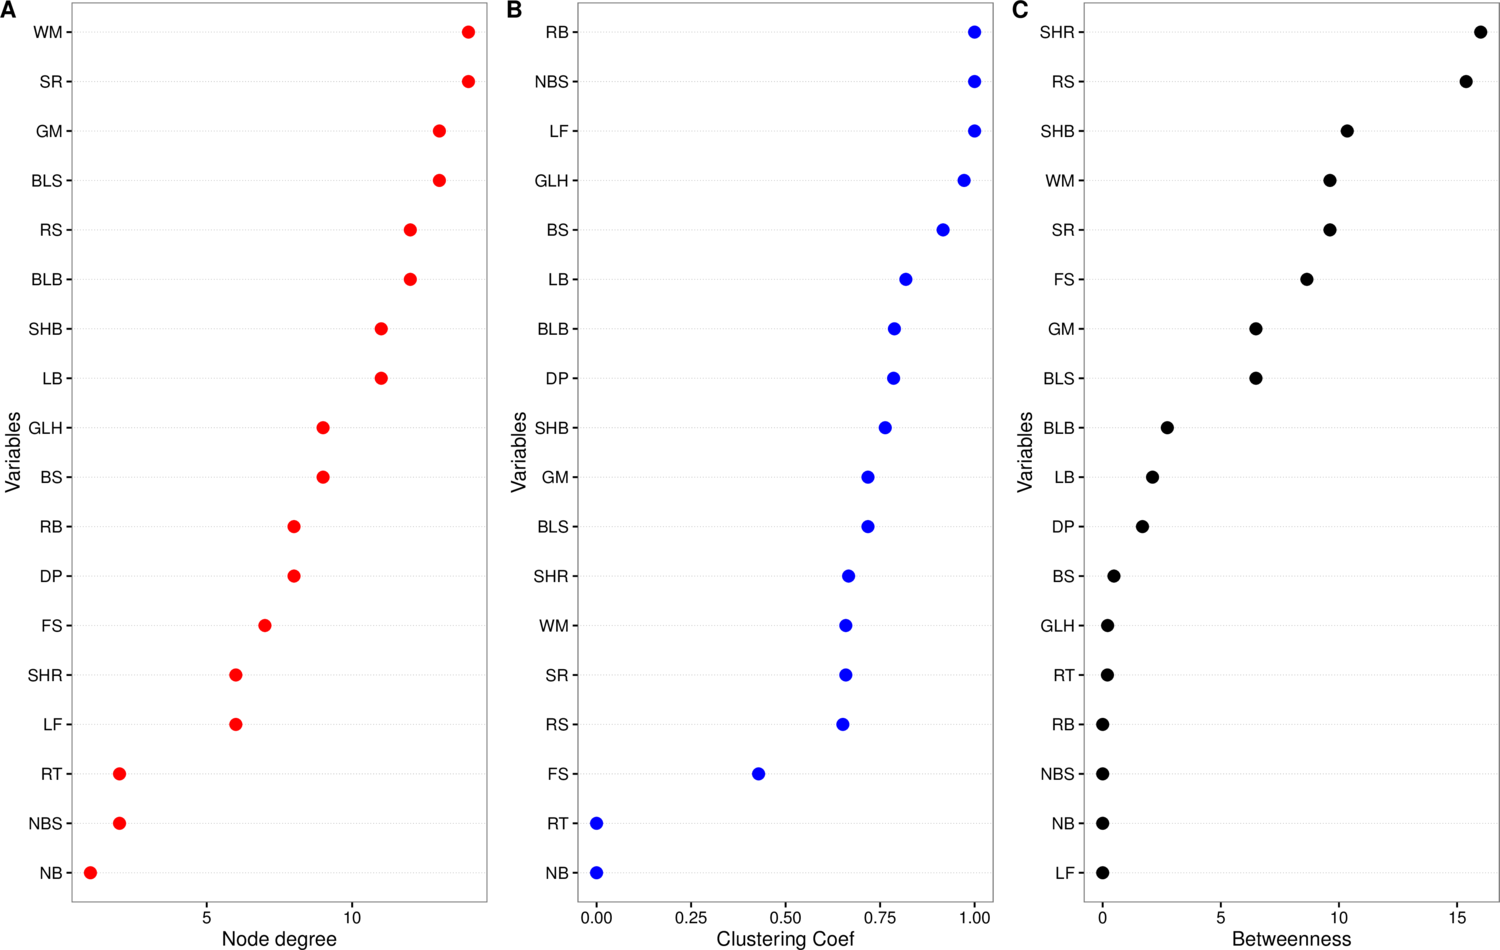
\includegraphics[width=\textwidth]{Network-analysis-/figures/nodeproptha_ws/nodeproptha_ws.png}


\paragraph{Makong Rive Delta, Vietnam}

Dry season network

MKD in dry season the network shows  20 variables (DH, BS, SR, SHB, NBS, SHR, GLH, and WH) showing  61 edges (significant pair-wise relationships).  The network reveals the three groups of injury profiles. The first group consisted of LB, DP, RB, DH, BS, and FS. The second group is composed of GLH, WPH, SR, WH, BPH, RS, WM. And the third group ( purple) consisted of RT, NB, SHB, BLB, LF, and NBS. The RB in the first group has high rank of betweenness and clustering coefficients. The injuries in the second group are relatively low betweenness, but high clustering coefficient, which indicated they are likely frequency to form complex association within the groups than forming between groups. In the third group BLB and NB have high rank of betweenness and they are associated with the injuries which have high betweenness. So the the first and the third group are like to more chance to form association between the groups, but less simple than the third group because of the average of the clustering coefficients.

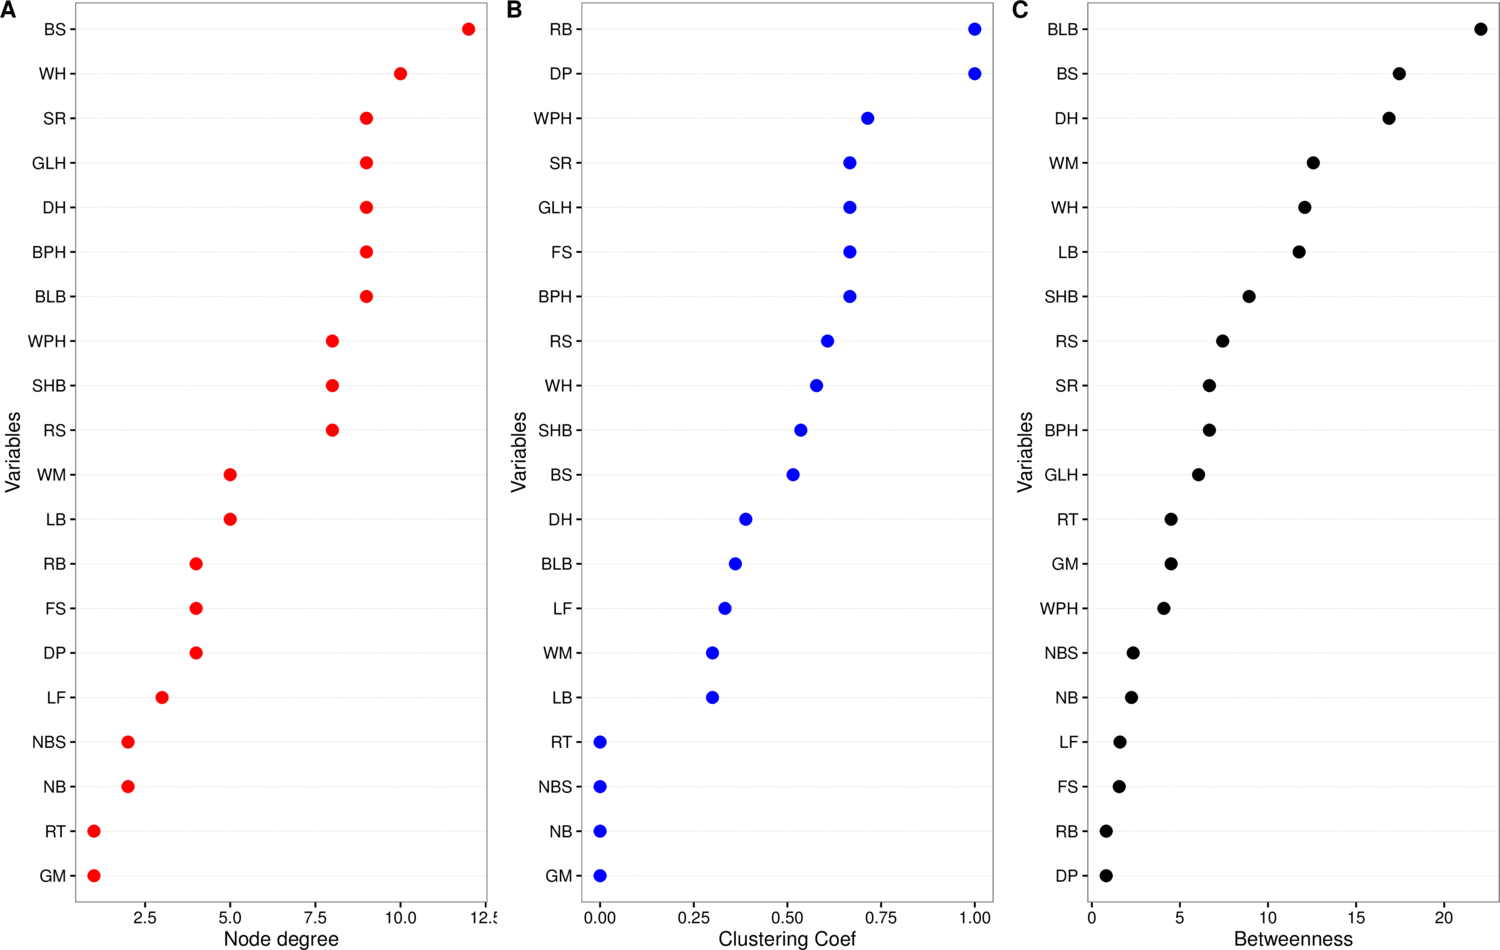
\includegraphics[width=\textwidth]{Network-analysis-/figures/nodepropvnm_ds/nodepropvnm_ds.png}

Wet season network

MKD in wet season the network shows  21 variables (DH, BS, SR, SHB, NBS, SHR, GLH, and WH) showing  54 edges (significant pair-wise relationships). From the structure of this network,, it seem to have two closely clustered groups base on optimal clustering algorithm. One group is composed of NB, SR, BS, WPH, RS, WM, DH, GLH, FS, RT.  Another group has BLB, BPH, LB, NBS, SHB, SHR, DP. The members with in clustered groups are relatively close in term of position based on  force layout.  The SHB and RB, RT, LB have high node degree and betweenness, whereas they are from different groups on injuries. They are probably more important in expressing co-occurrence within the group, or between groups. If they occurred, it is possible to  be able to observed the multiple injuries in this season.
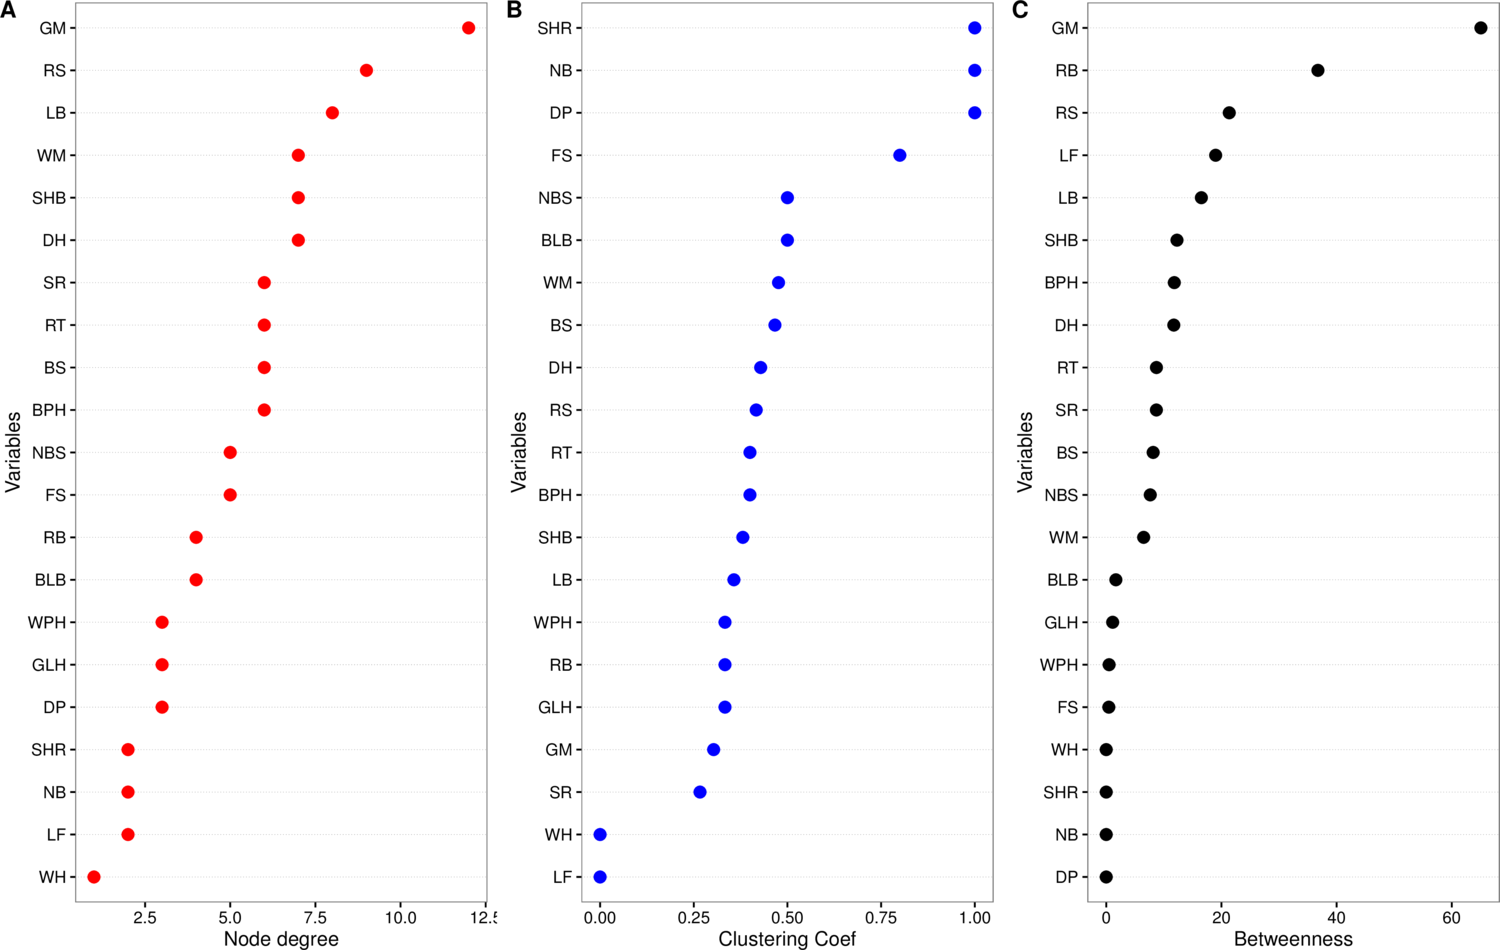
\includegraphics[width=\textwidth]{Network-analysis-/figures/nodepropvnm_ws/nodepropvnm_ws.png}

\begin{table} 
    \begin{tabular}{ c c c c c c c c c c c }
    \hline
         Country & Node & Link & Diameter & Connectivity & Geodesic & Density & Smallworldness & Centrality & Heterogeneity \\ 
         \hline
         India & 10 & 17 & 1.38 & 0.55 & 2.02 & 0.14 & 1.71 & 0.14 & 0.51 \\
         Indonesia & 22 & 48 & 1.40 & 0.46 & 2.25 & 0.06 & 1.24 & 0.07 & 0.64 \\
         Philippines & 21 & 33 & 1.85 & 0.28 & 2.26 & 0.07 & 0.82 & 0.19 & 0.89 \\
         Thailand & 18 & 63 & 1.11 & 0.47 & 1.81 & 0.15 & 1.07 & 0.20 & 0.70 \\
         Vietnam & 20 & 47 & 1.24 & 0.53 & 2.05 & 0.08 & 1.27 & 0.08 & 0.47 \\ 
     \hline  
    \end{tabular} 
    \caption{Network statistics for network graph each country}
\label{table:Network_stat}
\end{table}

%=== Here is the temp files
